\chapter{Flow entry verification}
This work focuses on the problem that a compromised switch will bring and presents the methods to detect such a switch. This work involves two parts: \textit{flow entry verification}. We will define the threat model that both parts share, and explain them along with their attack scenarios and detection algorithms.

\section{Threat model and Attack scenario}
In this work, we assume the following scenario of compromising a switch in the threat model:
\begin{enumerate}
\item
Only one OpenFlow switch is compromised. No cooperation among multiple compromised switches for attacks will happen.
\item
The switches are able to access the Internet. 
\item
Other parts of the network such as the controller, other switches and hosts function normally. Any potential flaw is unintentional and out of the scope of this work.
\item
An attacker cannot totally change the way of switch processing or core mechanism, but only perform the attack by modifying flow entries.
\item
Initially, the network is all clean, and nothing is compromised. The attacks take place some time after the whole network is established.
\end{enumerate}

The attack scenarios beyond the assumptions such as multiple compromised switches, as well as possible circumvention, will be discussed in Section~\ref{Further_discussion}.

\section{Flow entry verification}
In the first part of this work, we propose a method to detect if the flow entries of a switch work as expected. The method is inspired by \cite{CKGL15}. The method in this work has two main enhancements. First, it reduces the number of detection packets required, and therefore increases the efficiency significantly. Second, no additional flow entries other than table-miss is needed, resulting in less effort for setting up and cleaning up.

\subsection{Detection method}
\label{Detection_method}
The main idea of the method is to assemble a packet that will go through a sequence of switches by matching the match fields in the flow entries of these switches. Then the packet will be sent into the network, go through the switches, and should be sent back to the controller finally if nothing goes wrong. Therefore, the detection packet can check whether the matched flow entries on these switches work as expected or not. For this purpose, we need to find \textit{the sequence of switches} that a detection packet should pass through, find the flow entry on each switch with which the packet will be matched, and set the fields in the packet so that it will pass through the switches in order. Because the controller has the network-wise visibility and the policy of all the flow entries, it is able to decide the sequence of switches to be involved and the detection packet in each run of detection.

The flow chart of the flow entry detection process in the controller is shown in Figure~\ref{flow_entry_detection_flowchart}. Let $S=\{s_1,s_2,\ldots,s_n\}$ be the set of switches under the control of a controller, and $f(s_i)$, where $i=1\ldots n$, represents the flow entries on $S_i$. Let $F=\cup_{i=1}^n f(s_i)$, i.e., the set of all the flow entries. In the first step, we attempt to find a partition $P$ of $F$, such that each element in $P$ (i.e., a subset of $F$), namely an \textit{aggregated group}, contains exactly one selected flow entry on each switch from a non-empty subset of $S$. The flow entry on each switch is selected according to the following two conditions, namely the \textit{aggregation conditions}, and it should have an output action that forwards the matched packets to the next switch.

\begin{figure}[H]
\begin{center} 
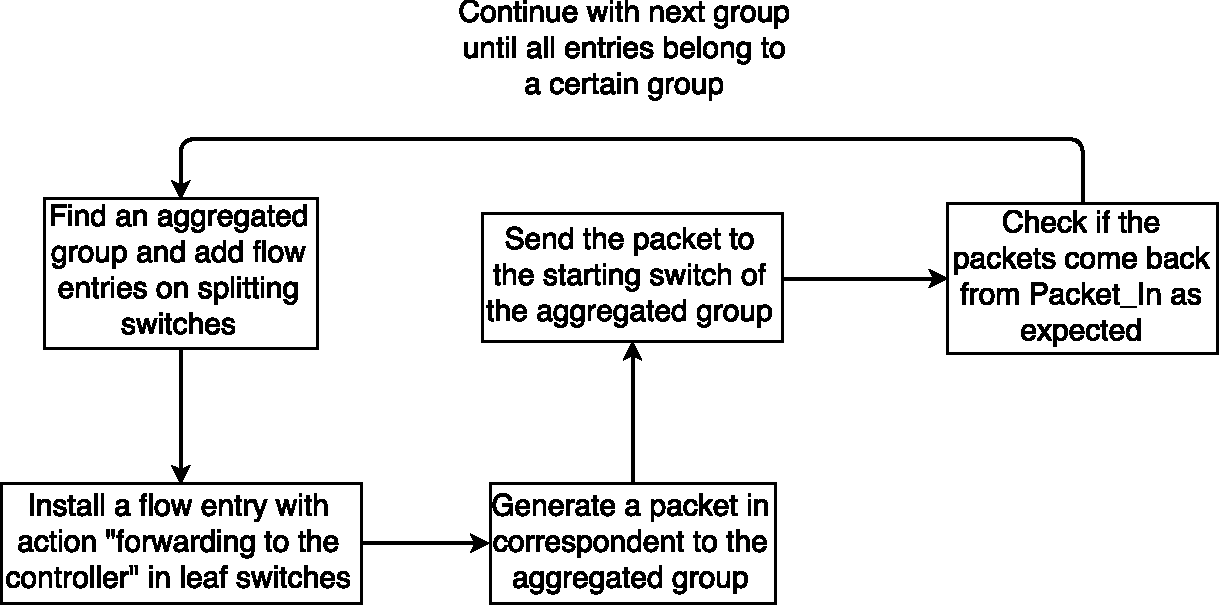
\includegraphics[width=1\textwidth]{figures/flow_entry_detection_flowchart.pdf}
\end{center}
\caption{The flow chart of the flow entry detection process.}
\label{flow_entry_detection_flowchart}
\end{figure}

\begin{enumerate}
\item
In the same group, the flow entries on different switches either have exactly the same match fields and values, or have no common match fields.
\item
A switch has at most one flow entry selected in the same group. 
\end{enumerate}

The aggregation conditions are defined to ensure a valid detection packet can be forged and sent through the switches. The first condition is the essential idea of the method: aggregating flow entries this way allows us to forge a packet with multiple fields that match the entries inside the same aggregated group. The second condition is to eliminate the cycle in the forwarding path of a detection packet. Since a switch has at most one flow entry in an aggregated group, a detection packet will not go through a switch more than once, and thus no forwarding loop can exist in the path.

A detection packet is forged according to the match fields of the flow entries in an aggregated group. In other words, each detection packet will pass through a sequence of switches whose selected flow entry makes up the aggregated group. The forged detection packets should also meet the dependency requirement stated in the third paragraph of \ref{SDN and OpenFlow}; otherwise, the packet will not be matched with any flow entry. The controller will sent the detection packet with PACKET\_OUT, the detection packet will pass through a sequence of switches with a flow entry in an aggregated group in order. Eventually, when the detection packet passes through the last switch in the aggregated group, it will be sent to a switch that does not contain any flow entry that matches the aggregation condition. As a result, the packet will fail to match any flow entry on that switch and be sent back to the controller due to the table-miss entry, notifying the controller that the detection process of this aggregated group is carried out as expected. 

When finding an aggregation group, we start from the first switch and try to find a flow entry that matches the aggregation conditions and has an output action to the second switch. We move on to the second switch and try to find an entry which also meets the requirement, and it has an output action action to the third switch, and so on. Eventually when we find a switch that does not contain any flow entry that fits the requirement, and the detection process in this aggregated group ends. Because all flow entries will be aggregated to some aggregated group, all the flow entries will be verified after all the aggregated groups have been explored.

Figure~\ref{aggregated_group} illustrates a realistic example with an aggregated group and the content of a constructed packet. The flow entries connected by arrows belong to the same group. The controller constructs a packet according to the match fields of flow entries inside the aggregated group. In the example figure, we have a controller, three switches, $s_a$,$s_b$ and $s_c$, and a packet to be constructed. Only the entries that will be matched are shown. In $s_a$, there is a flow entry that contains match field \texttt{eth\_dst}=\texttt{a2:b4:c6:d8:e0:f1} and an output action to $s_b$. In $s_b$, the flow entry has match fields \texttt{eth\_type}=\texttt{0x800}, \texttt{ipv4\_src}=\texttt{140.123.103.123} and an output action to $s_c$. The \texttt{eth\_type}=\texttt{0x800} is required for a valid IP match field. According to the match fields of these flow entries in the aggregated group, the forged detection packet will contain \texttt{eth\_dst} as \texttt{a2:b4:c6:d8:e0:f1}, \texttt{ipv4\_src} as \texttt{140.123.103.123}. No flow entry belongs to this aggregated group in $s_c$. Therefore, the packet is sent to $s_a$, goes through $s_b$, and sent back to the controller by table-miss entry in $s_c$. 

\begin{figure}[H]
\begin{center}
\includegraphics[width=1\textwidth]{figures/aggregated_group.png}
\end{center}
\caption{An aggregated group and constructed packet. \red{wrong figure}}
\label{aggregated_group}
\end{figure}

The process of generating a packet is done along with defining one aggregated group. Its pseudo-code is as follows:

\begin {tcolorbox}[blanker,float=tbp,
grow to left by=1cm, grow to right by=1cm]
\begin{algorithm}[H]

  \caption{Packet generating process.}
  \begin{algorithmic}[1]
    \Require
      Set of switch, $switches$;  \newline
      Each switch is a set of entries, $switch$;  \newline
      Info of an entry, including match field, value and destination switch, $entry$;  \newline
      Visited status of every switch in one group finding process, cleared every round, $visited\_switch$;  \newline
      An under-constructing packet that is initially empty and send after one round of group finding is done, $packet$; \newline
      In-Degree of every switch that will be alternated dynamically, $switch_in_degree$
      
    \Function{find\_aggregated\_groups}{$switches$}
      \State $\textit{group\_id} \gets 0$;
      \While{not all $switch$ is empty}  
            \State $\textit{starting\_switch} \gets A\;switch\;with\;max\;\Call{heuristic}{\textit{switch}}\;\forall\;\textit{switch} \in \textit{switches}$;
            \State $\textit{packet} \gets empty\;dictionary$;   // Cleared per group finding round
            \State $packet[vid] \gets \textit{group\_id}$;   // Use vid as group identifier 
            \State $group\_id \gets \textit{group\_id} + 1$;
            \State $\textit{packet} \gets \Call{find\_one\_group}{\textit{starting\_switch}, \textit{packet},$visited\_switch$}$;
            \State $Send\;\textit{packet}\;with\;PACKET\_OUT$;
      \EndWhile
    \EndFunction
    \State
    \Function{heuristic}{$switch$}
      \State \Return $value$;
    \EndFunction
    \State
  \algstore{find_group}
  \end{algorithmic}
\end{algorithm}
\end{tcolorbox}

\begin {tcolorbox}[blanker,float=tbp,
grow to left by=1cm, grow to right by=1cm]
\begin{algorithm}[H]
  \begin{algorithmic}[1]
  \algrestore{find_group}
    \Function{find\_one\_group}{switch$, packet$, $visited\_switch$}
      \State $\textit{best\_entry} \gets \textit{entry}\;with\;max\; \Call{heuristic}{\textit{entry}[\textit{dst\_switch}]}\;\forall\;\textit{entry}\;in\;\textit{switch}$
      \State $such\;that\;\textit{entry}[\textit{dst\_switch}] \notin \textit{visited\_switch}\;and\;\textit{entry}\;fit\;in\;group$;  //get best entry that fits the aggregation conditions;
      \If{$best\_entry$}  //found an entry that satisfy aggregation condition
        \State $\textit{packet}[\textit{match\_field}] \gets \textit{match\_value}$;  //add match field to detection packet
        \State Add $best\_entry$[$dst\_switch$] to $visited\_switch$;
        \State \Return \Call{packet\_gen}{$match\_field$, $match\_value$, $action$, $packet$};  //no entry in the switch satisfies aggregation condition of this group
      \EndIf
      \State \Return $packet$;
    \EndFunction
  \end{algorithmic}
\end{algorithm}
\end{tcolorbox}

One detection packet is required for each aggregated group, so minimizing the number of aggregated groups means minimizing the number of detection packets, resulting in fast detection. Given the above aggregation condition, we want to \textit{look for the minimized partition of aggregated groups from} $F$. As the abstraction of the problem, we treat switches as vertices and forwarding actions as edges. It forms a complex DAG problem and is more complex than the longest path problem \cite{DMR97,RU04}, which is NP-complete and hard to find a approximation algorithm. We use A* search to deal with the problem. While we are trying to find a fitting entry in the aggregated group defining process, the forwarding destination switch of entries is extracted and evaluated by a heuristic function, which becomes the heuristic value of that entry. The entry with highest heuristic value will be selected and removed from the graph abstraction.

Talk about hueristic function here XXXXXXXXXXXXXXXXXXXXXX
XXXXXXXXXXXX Inspired by Euler Path, the number XXXXXX. The reason behind the thought is that, the vertex which is treated as the destination the least time should be used as start point in order to reduce the number of necessary groups.
XXXXXXXXXXXXX

\subsection{Further discussion of attack scenario and our method}
\label{Further_discussion}

The trait of match field mentioned in thrid paragraph of \ref{SDN and OpenFlow} makes match field aggregation much more complicated. These kind of situations can still be covered by our method with some modification if we manage to resolve the complex conjunctive conditions. Take the entry with multiple match fields for example, if all the fields and values match the under-constructing packet, we process it according to first aggregation rule. Otherwise we fill the packet with all of those match fields. If any match field is already taken with different value, it will be ignored for this turn of aggregation process and fill the match fields in another packet that has no conflict field. However, the main purpose of our method is to show the effectiveness of flow entry aggregation method. We will demonstrate with the most simple condition, which is that every entry has only one matching field and use only one flow table.

It is certainly possible that more than one switch are made by the same manufacturer or have the same software version in the same network, so multiple switches share the same vulnerabilities and may be compromised simultaneously. However, cooperation between multiple compromised switches complicates the scenario significantly. In order to simplify the case as a starting point for developing the detection method, we assume only one switch inside the network is compromised.

Suppose an attacker is able to add, remove, or modify the entries in the flow tables of a compromised
switch without notifying the controller, so packets may be forwarded to an undesired destination. The proposed method is intended to detect this behavior with high efficiency. In this method, only output action of packets is considered. Other actions such as dropping packets, setting field, changing TTL is not included \sout{\red{Cann't they (e.g., dropping packets) be detected?}}. Although there are might be reasonable ways to deal with these actions, for example, to detect packet dropping, we can add timeout checking function, such detection function is irrelevant to our main method and is not implemented in our work.

In this detection method, there is another important consideration: the controller must maintain unpolluted information of all flow entries. It is not reliable for a controller to obtain flow entry information by querying switches because a switch may be malicious and forge a fake response that gives false information about the flow entries. That is the reason for the last statement of attack model. Also mind that the detection packet should not be distinguishable from normal packet, otherwise the attacker will be able to circumvent the detection method. 
